\chapter{\label{chap:entwurf}Konzeption}
% ### Design ###
\section{Das Design}
Aus den Anforderungen in Kapitel \ref{chap:anforderungen} entsteht Design. Erfüllt Kriterien... Aktuelle Geschwindigkeit nicht relevant, bzw Erhöhung auf gewisse km/h auch nicht. Differenz ist beim Fahrrad nicht so hoch wie beim Auto.\\
auf schwarzem Hintergrund wirken Farben intensiver und leuchtender = sind besser aus dem Augenwinkel identifizierbar.\\
Eingreifempfehlung: Farbe Hellblau gewählt.\\
Zeichen sind eindeutig und auch bei Farbenblindheit oder rot/grün schwäche identifizierbar.
\begin{figure}[H]
        \centering
           \begin{subfigure}[t]{0.23\textwidth}
                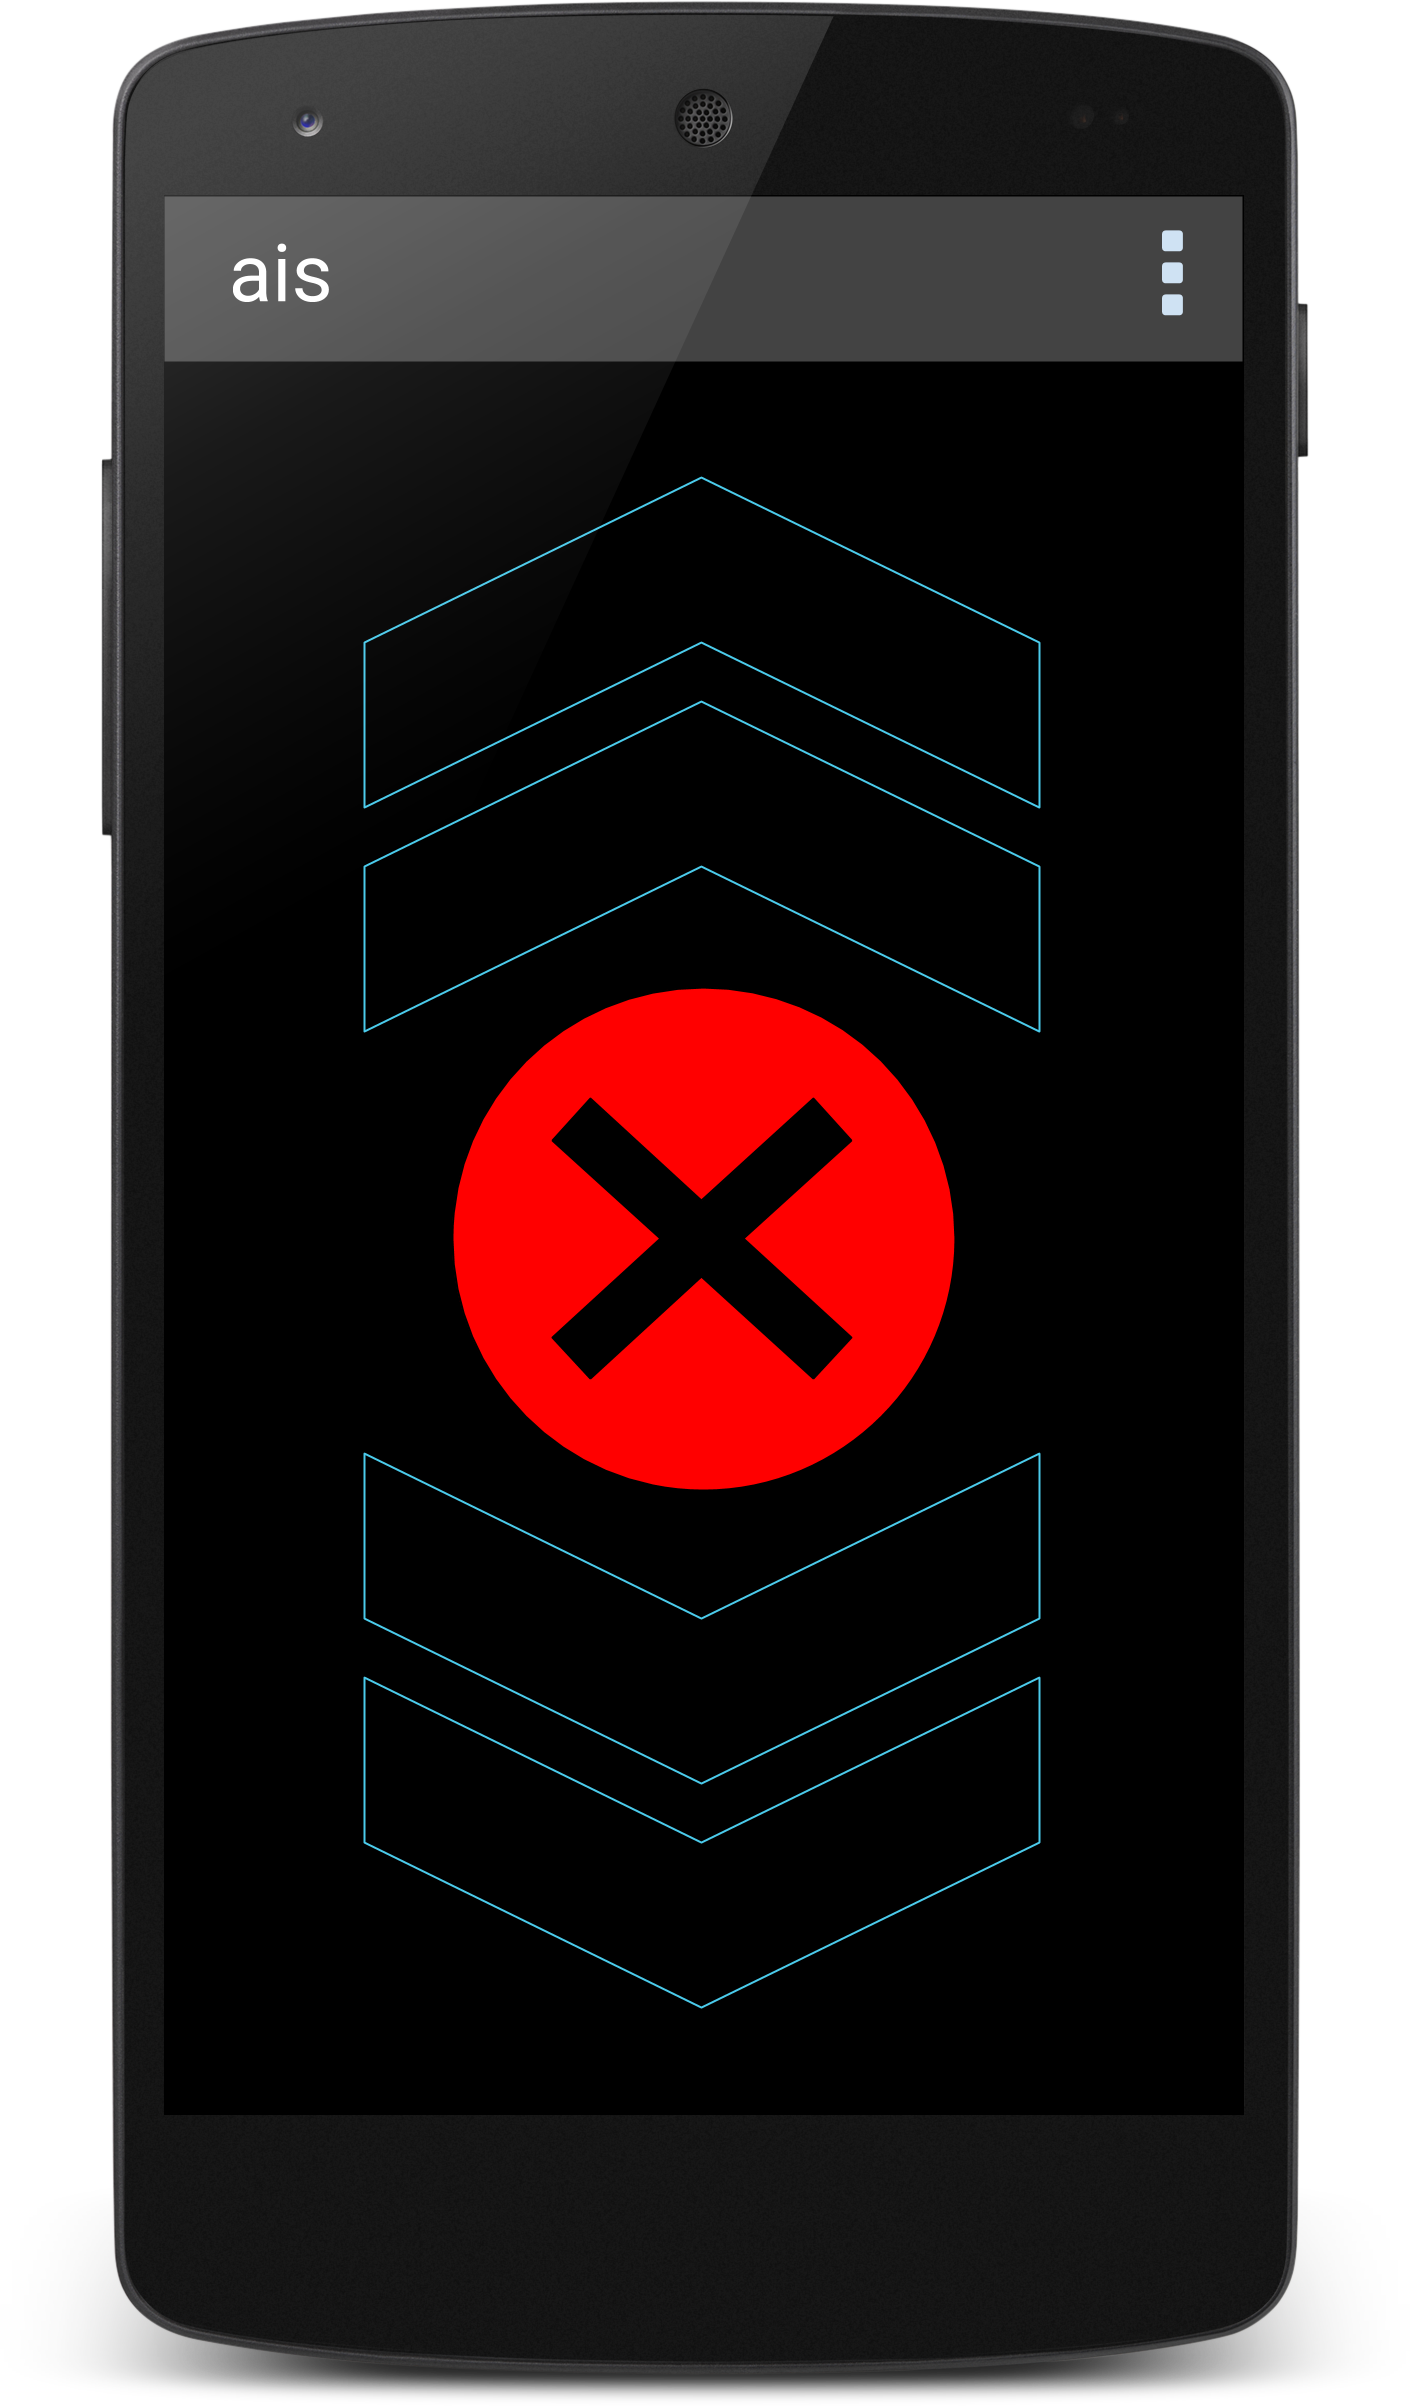
\includegraphics[width=\textwidth]{stop}
                \caption[Systemzustand d]{keine Weiterfahrt möglich}
                \label{fig:stop}
        \end{subfigure}
           ~ 
              \begin{subfigure}[t]{0.23\textwidth}
                
\includegraphics[width=\textwidth]{yeah}
                \caption[Systemzustand c]{Kein Aktionsbedarf}
                \label{fig:yeah}
        \end{subfigure}
           ~
        \begin{subfigure}[t]{0.23\textwidth}
                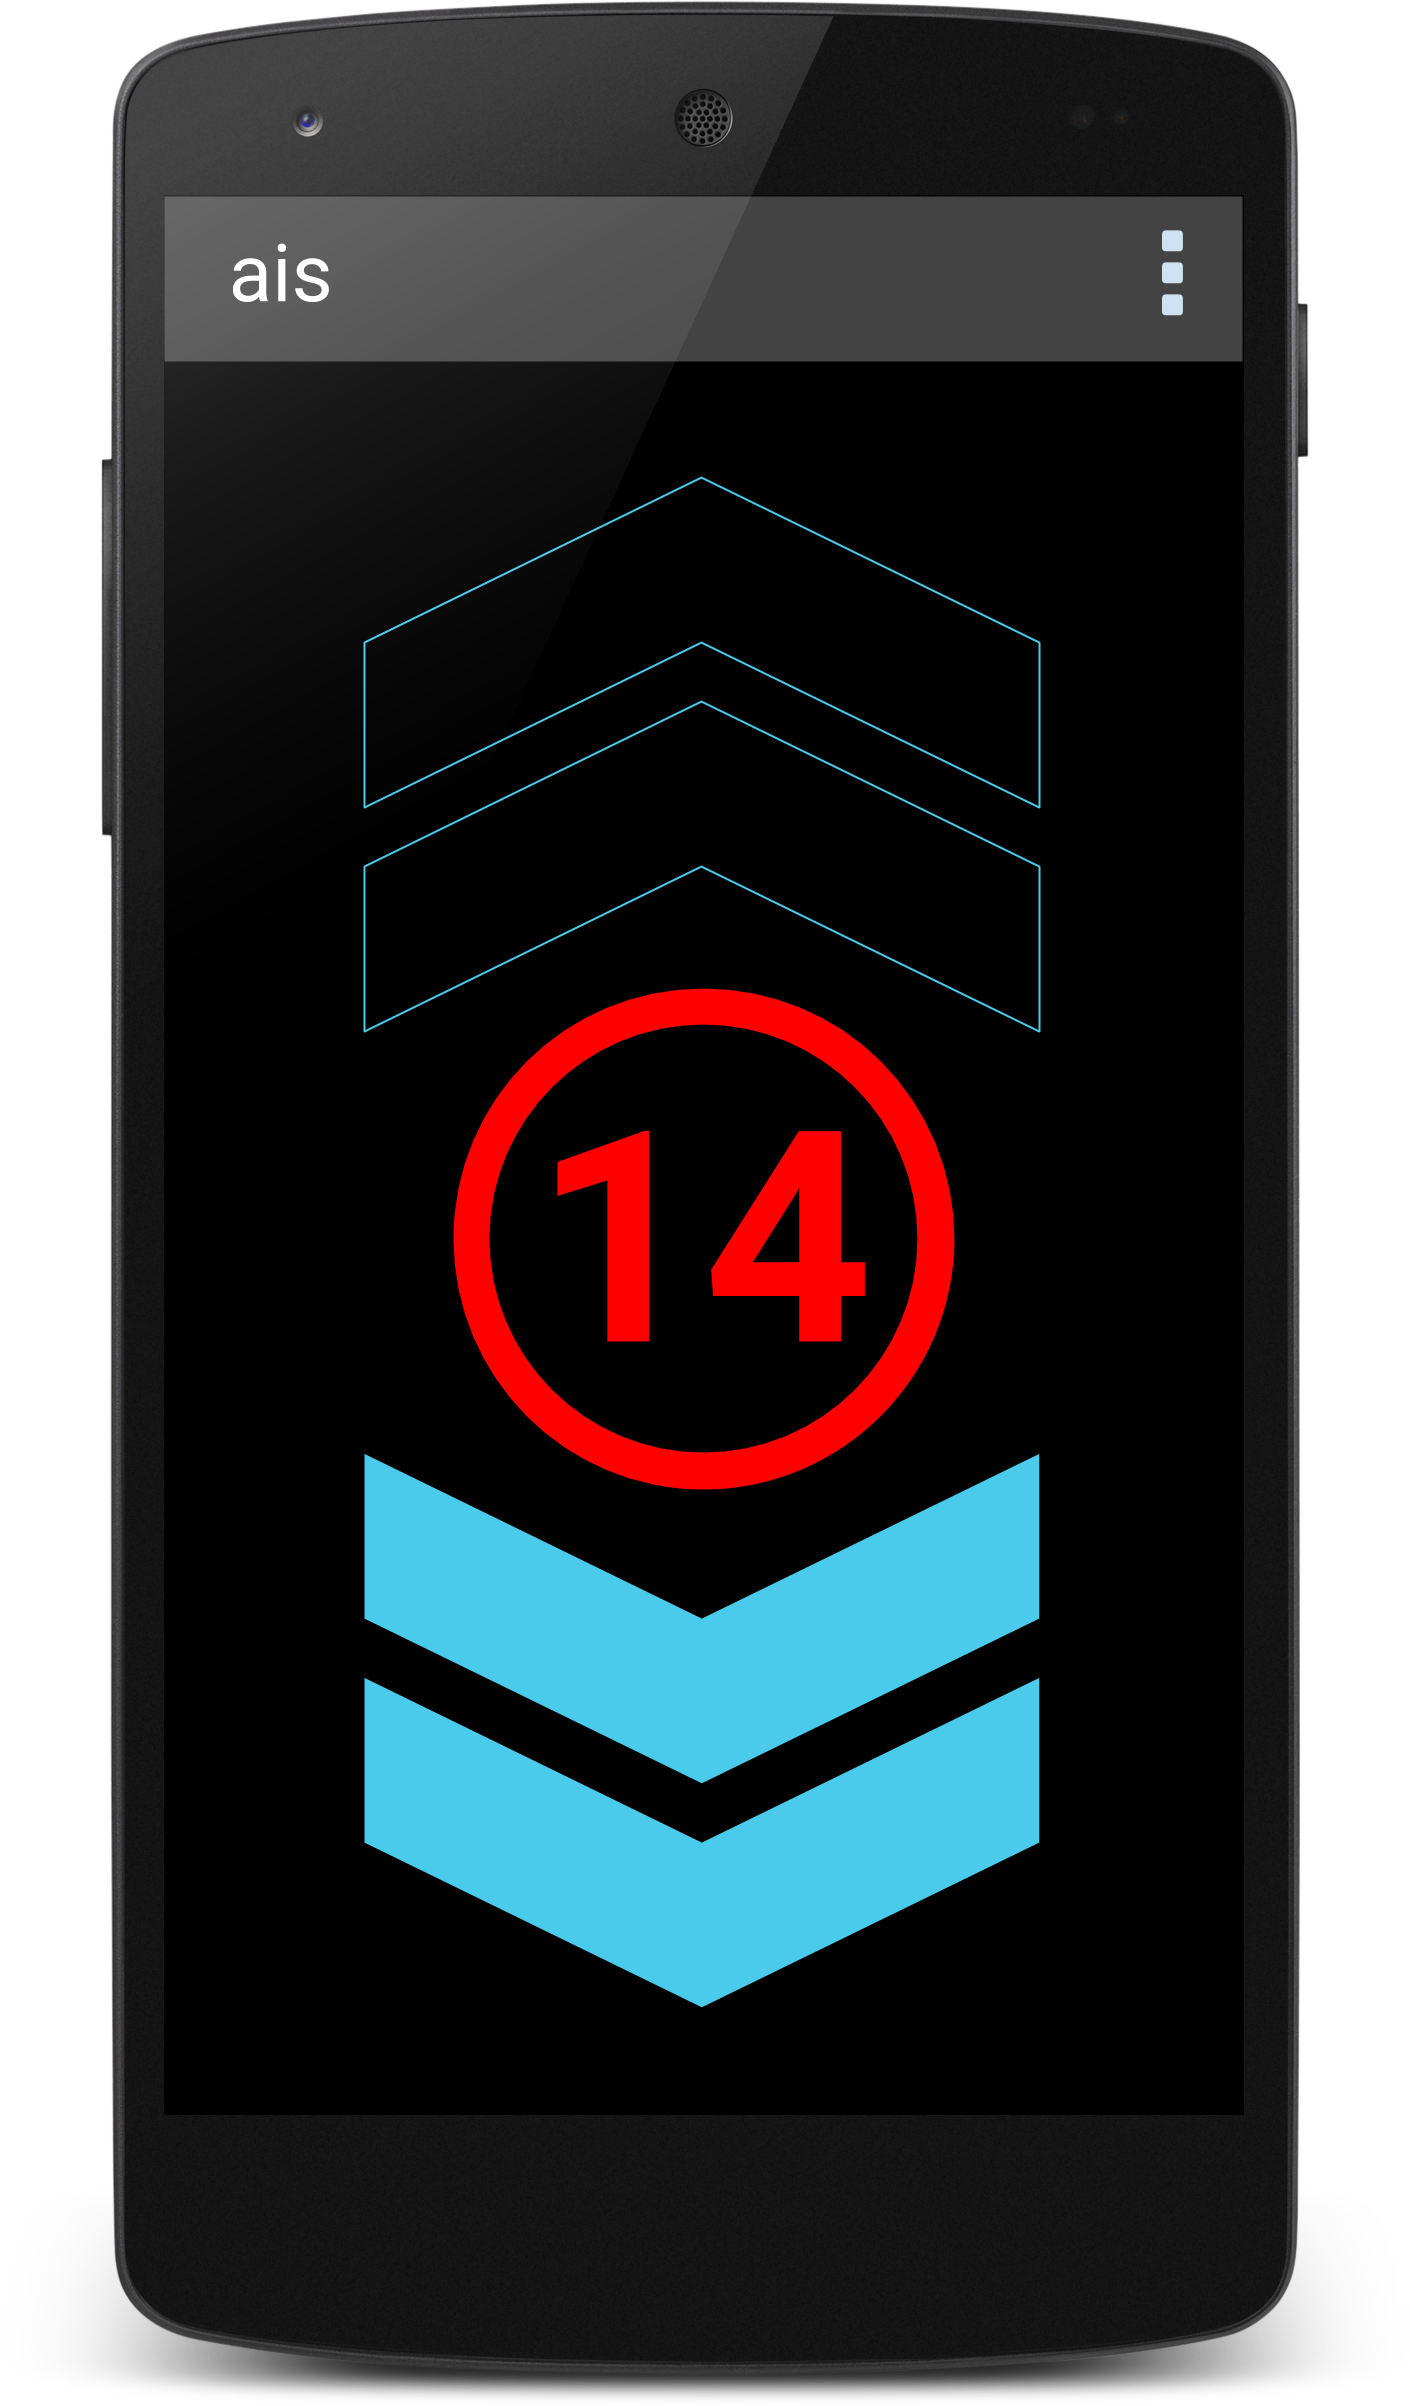
\includegraphics[width=\textwidth]{langsamer0}
                \caption[Systemzustand a]{Weiterfahrt durch Verlangsamung  möglich}
                \label{fig:langsamer}
        \end{subfigure}
        ~
        \begin{subfigure}[t]{0.23\textwidth}
                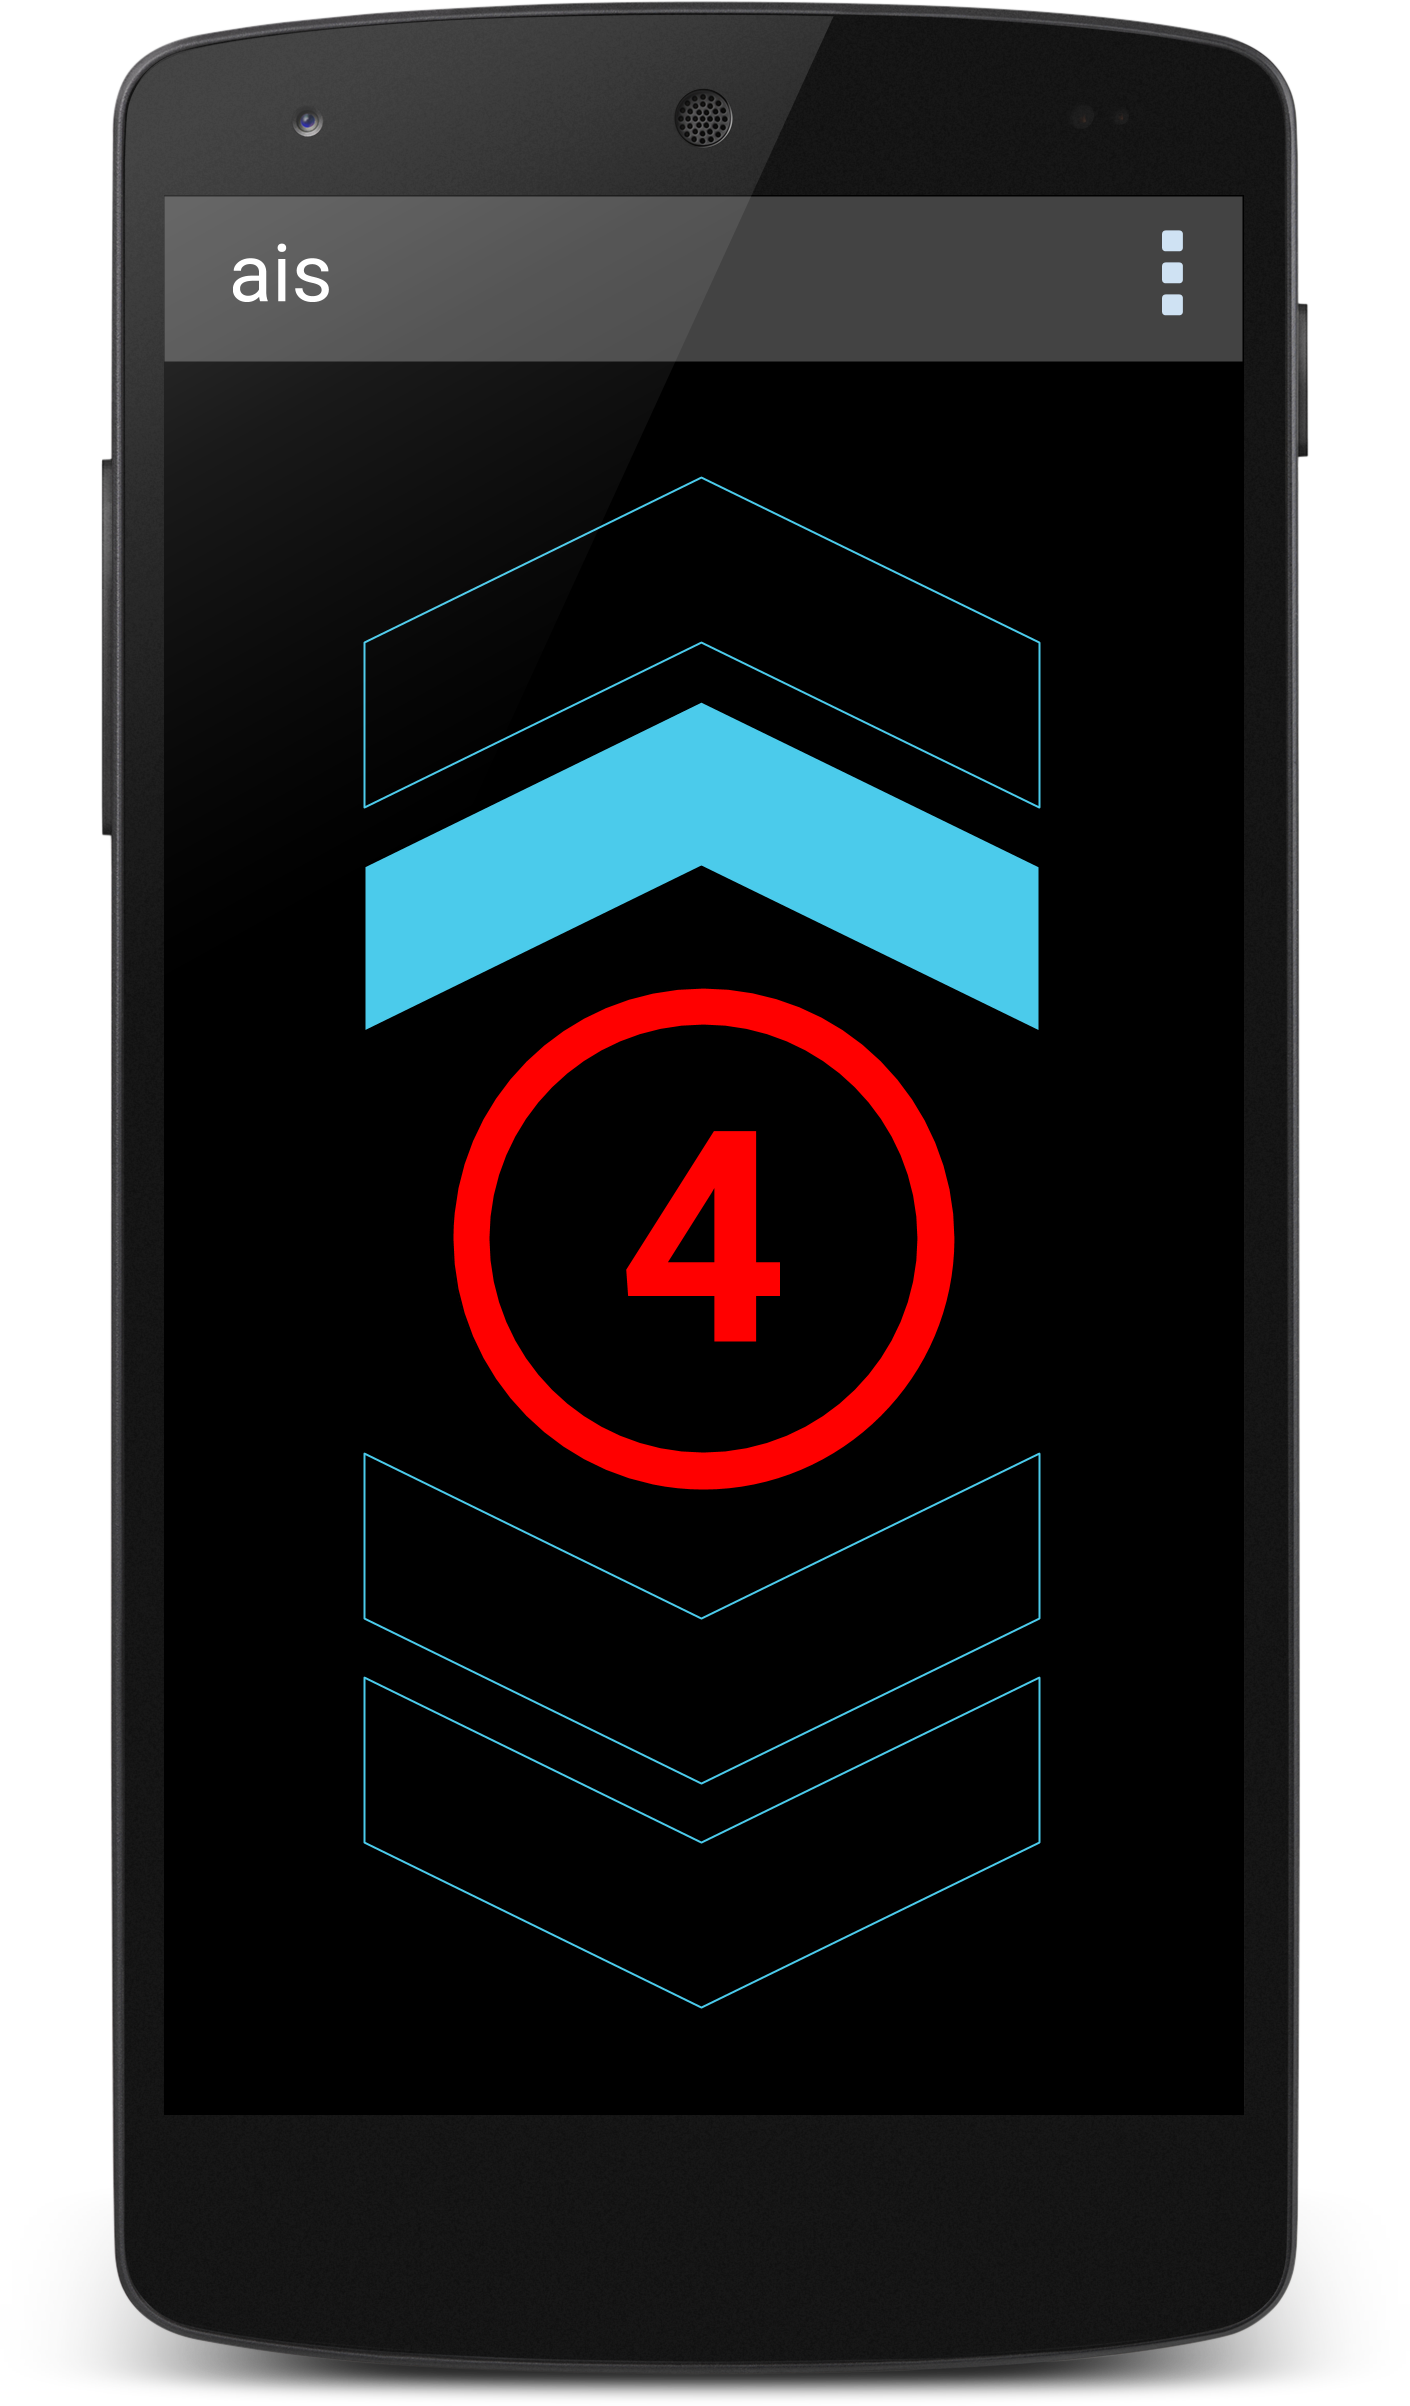
\includegraphics[width=\textwidth]{schneller0}
                \caption[Systemzustand b]{Weiterfahrt durch Beschleunigung möglich}
                \label{fig:schneller}
        \end{subfigure}     
        \caption[Systemzustände im Ampelbereich]{Entwurf des Designs anhand der Systemzustände}
        \label{fig:mockup}
\end{figure} 
\subsection{Anzeigeelemente}
\subsubsection{Geschwindigkeit}
\subsubsection{Ampeln}
\subsubsection{Informationen}
% ### Achitektur ###
\section{Architektur}
Klassenstruktur..
\section{Ampeldatenanfrage und Auswertung}
\section{Theorie}
Um die korrekte Umsetzung des Prototyps zu ermöglichen, müssen zunächst einmal prinzipielle
Theorien und Hintergründe diesen betreffend betrachtet werden.
grundlegendes Wissen über geographische Koordinaten sowie mathematische Voraussetzungen im Umgang mit diesen, müssen zur Ideenverwirklichung berücksichtigt werden.
\subsection{Die Berechnung der Entferung}
\subsection{Die Berechnung der Ankunft in Abhängigkeit der Geschwindigkeit}
\subsection{Die Anzeige der Restrotanzeige}
